\documentclass[conference]{IEEEtran}
\IEEEoverridecommandlockouts

\usepackage{cite}
\usepackage{amsmath,amssymb,amsfonts}
\usepackage{booktabs}
\usepackage{graphicx}
\usepackage{tikz}
\usepackage{pgfplots}
\usepgfplotslibrary{groupplots}
\pgfplotsset{compat=1.18}
\usetikzlibrary{arrows.meta,positioning,shapes.geometric}
\usepackage{hyperref}
\hypersetup{hidelinks}

\begin{document}

\title{An Integrated ROS\,2 Ackermann Vehicle Stack for Scaled Autonomous Navigation:\
Simulation, Planning, Control, Localization, and Embedded Actuation}

\author{
\IEEEauthorblockN{Andrew Abdelmalak}
\IEEEauthorblockA{\textit{Dept. of Mechatronics Engineering}\\
\textit{German University in Cairo}\\
Cairo, Egypt\\
andrew.abdelmalak@student.guc.edu.eg}
\and
\IEEEauthorblockN{Daniel Boules}
\IEEEauthorblockA{\textit{Dept. of Mechatronics Engineering}\\
\textit{German University in Cairo}\\
Cairo, Egypt\\
daniel.boules@student.guc.edu.eg}
\and
\IEEEauthorblockN{David Girgis}
\IEEEauthorblockA{\textit{Dept. of Mechatronics Engineering}\\
\textit{German University in Cairo}\\
Cairo, Egypt\\
david.girgis@student.guc.edu.eg}
\and
\IEEEauthorblockN{Kirolous Kirolous}
\IEEEauthorblockA{\textit{Dept. of Mechatronics Engineering}\\
\textit{German University in Cairo}\\
Cairo, Egypt\\
kirolous.kirolous@student.guc.edu.eg}
\and
\IEEEauthorblockN{Samir Yacoub}
\IEEEauthorblockA{\textit{Dept. of Mechatronics Engineering}\\
\textit{German University in Cairo}\\
Cairo, Egypt\\
samir.yacoub@student.guc.edu.eg}
\and
\IEEEauthorblockN{Youssef Salama}
\IEEEauthorblockA{\textit{Dept. of Mechatronics Engineering}\\
\textit{German University in Cairo}\\
Cairo, Egypt\\
youssef.salama@student.guc.edu.eg}
}

\maketitle

\begin{abstract}
Many scaled-vehicle projects stop at ROS bring-up, teleoperation, or isolated
localization experiments, leaving the full autonomy pipeline only partially
validated. This paper presents the final integrated stack built by Team~23 for a
scaled Ackermann vehicle using ROS\,2 Jazzy, Gazebo Harmonic, Python planning
and control nodes, a Raspberry Pi~4 host, and a Raspberry Pi Pico-based
embedded actuation layer. The final system connects three structured track
scenarios to a shared planner, a PID longitudinal controller, a Stanley-style
lateral controller, and a linearized Kalman-filter localization node. In the
exported Milestone~5 simulation artifacts, with injected measurement noise of
$0.03$~m in position, $0.04$~rad in heading, $0.05$~m/s in speed, and
$0.08$~rad/s in yaw rate, the filter reduces position root-mean-square error
from $4.17$~cm to $0.71$~cm on the straight track and to $0.69$~cm on the
racing track, while heading root-mean-square error drops from $2.19^{\circ}$ to
$0.42^{\circ}$ in both cases. Hardware demonstrations confirm that the same
high-level pipeline can run headlessly on the physical platform for predefined
straight, obstacle-avoidance, and city-style tracks. The main limitation is
that the system is validated on known tracks with proprioceptive sensing only,
not in generalized obstacle-rich environments.
\end{abstract}

\begin{IEEEkeywords}
ROS 2, Ackermann steering, autonomous vehicle, path planning, Kalman filtering
\end{IEEEkeywords}

\section{Introduction}
\label{sec:intro}

Scaled autonomous vehicles are useful precisely because they expose the same
integration problem faced by larger platforms: middleware, control, planning,
state estimation, and embedded actuation must share a consistent command-state
interface before autonomy claims are meaningful. For Ackermann vehicles, that
integration is further constrained by nonholonomic steering geometry, limited
sensing, and the dynamics mismatch between simulator-friendly models and small
physical chassis \cite{ROS2JazzyDocs,GazeboHarmonicDocs,Xu2023}.

The literature covers each major subsystem independently. ROS\,2 and Gazebo
provide the middleware and simulation backbone for modular robotic systems
\cite{ROS2JazzyDocs,GazeboHarmonicDocs}. Stanley-based lateral control remains a
practical choice for Ackermann path tracking because it combines heading and
cross-track correction in a compact law \cite{Hoffmann2007}. Kalman-based sensor
fusion is also well established for vehicle localization when encoder and
inertial measurements must be combined \cite{Peiris2024,Georgiev2025}. The gap,
however, is not algorithm availability; it is showing a single low-cost stack
that carries shared interfaces from simulation bring-up to planning, control,
embedded actuation, and localization demonstrations on one platform.

This paper presents Team~23's final MCTR~1002 autonomous systems project as an
integrated autonomy pipeline rather than a milestone checklist. The development
process was milestone-based, but the final contribution is the connected stack
shown in Fig.~\ref{fig:stack_architecture}. The paper makes four project-level
contributions:

\begin{enumerate}
  \item it documents a unified ROS\,2 Jazzy Ackermann stack spanning Gazebo
        simulation, shared planning and control nodes, Raspberry Pi host-side
        execution, and Pico-based embedded actuation and sensing;
  \item it shows that the final value lies in the end-to-end autonomy pipeline,
        not ROS bring-up alone, by connecting validation, planning, control,
        localization, and hardware demonstrations into one consistent workflow;
  \item it provides source-backed quantitative evidence from the exported MS5
        localization artifacts, including up to $83.5\%$ position-RMSE
        reduction and about $81\%$ heading-RMSE reduction under the documented
        noise settings;
  \item it states the observed limitation directly: the platform demonstrates
        autonomy on predefined tracks with limited sensing, not generalized
        autonomy in dynamic, obstacle-rich scenes.
\end{enumerate}

The remainder of the paper is organized as follows. Section~\ref{sec:related}
summarizes the most relevant technical context. Section~\ref{sec:architecture}
presents the integrated system architecture. Section~\ref{sec:setup} describes
the vehicle platform and experimental setup. Section~\ref{sec:methods} covers
planning, control, and localization. Section~\ref{sec:results} reports the
results. Section~\ref{sec:discussion} interprets those results and states the
limitations. Section~\ref{sec:conclusion} concludes the paper.

\section{Related Work}
\label{sec:related}

ROS\,2 is a natural fit for staged robotics development because the DDS-based
publish-subscribe model decouples sensing, planning, control, and hardware
interfaces into reusable nodes \cite{ROS2JazzyDocs}. Gazebo Harmonic complements
that workflow by providing simulated sensors, actuators, and vehicle worlds that
can be exercised before hardware deployment \cite{GazeboHarmonicDocs}.

For Ackermann steering, the essential geometric relationship remains the shared
instantaneous center of rotation across the steered wheels. This is commonly
approximated with the kinematic bicycle model, which is accurate enough for low-
to moderate-speed scaled platforms and remains a useful basis for controller
design \cite{Xu2023}. Stanley tracking is still attractive in this setting
because heading error is handled explicitly instead of being hidden inside a
lookahead heuristic \cite{Hoffmann2007}.

Sensor fusion for small autonomous vehicles is also well established. Encoder and
IMU fusion improves the consistency of dead-reckoning trajectories by combining
the smooth short-term heading response of inertial sensing with the translational
constraints implied by wheel motion \cite{Peiris2024,Georgiev2025}. The present
work does not propose a new planner or estimator; it shows how these known
components can be assembled into a coherent ROS\,2 autonomy stack and evaluated
with honest scope boundaries.

\section{Integrated System Architecture}
\label{sec:architecture}

Figure~\ref{fig:stack_architecture} summarizes the final stack. The key design
decision is that simulation and hardware share the same high-level planner,
longitudinal controller, lateral controller, and filtered odometry interface.
Gazebo publishes ideal odometry into the localization node during simulation,
while the physical platform supplies encoder and IMU telemetry through the Pico.
The planner consumes filtered odometry and publishes desired speed, lane, and
heading targets. The speed controller converts the desired speed into a bounded
longitudinal command, and the Stanley-style lateral controller converts the lane
and heading targets into steering action. The command path then terminates either
at Gazebo through \texttt{ros\_gz\_bridge} or at the physical vehicle through a
USB serial link.

\begin{figure*}[t]
  \centering
  \resizebox{\textwidth}{!}{%
  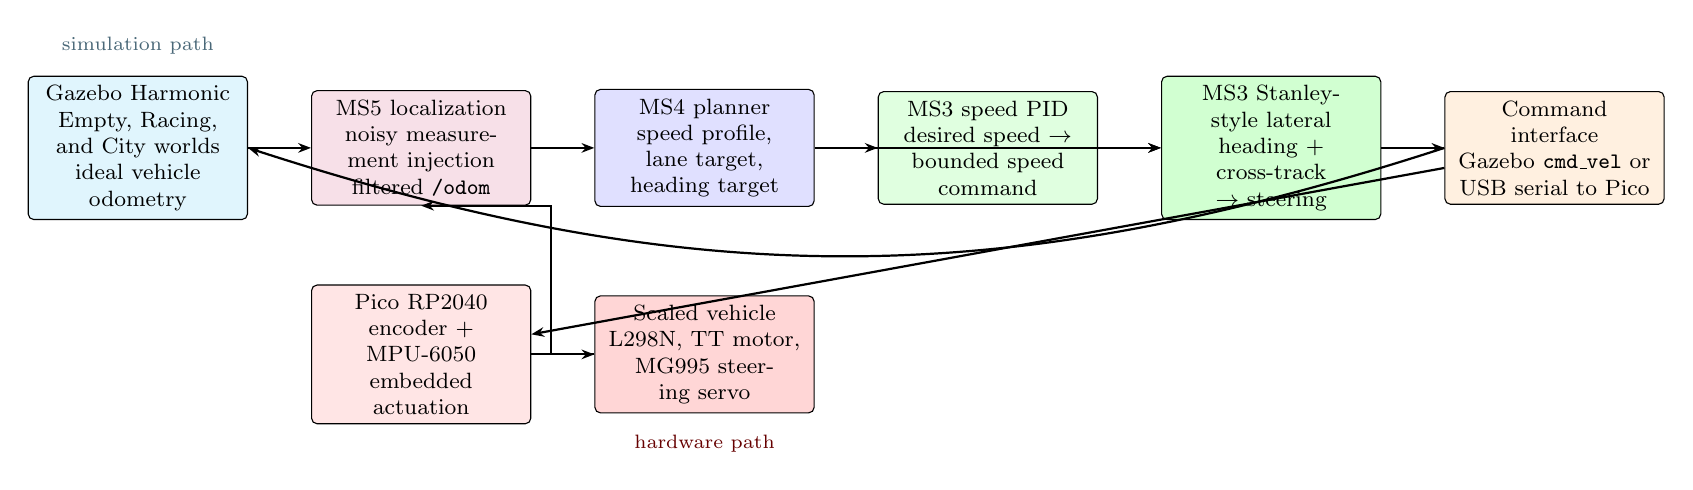
\begin{tikzpicture}[
    node distance=0.7cm and 0.8cm,
    box/.style={draw, rounded corners=2pt, align=center, minimum height=1.0cm,
      text width=2.55cm, font=\footnotesize},
    arrow/.style={-{Stealth[scale=0.7]}, thick}
  ]
    \node[box, fill=cyan!12] (sim) {Gazebo Harmonic\\
    Empty, Racing, and City worlds\\
    ideal vehicle odometry};
    \node[box, right=of sim, fill=purple!12] (loc) {MS5 localization\\
    noisy measurement injection\\
    filtered \texttt{/odom}};
    \node[box, right=of loc, fill=blue!12] (plan) {MS4 planner\\
    speed profile, lane target,\\
    heading target};
    \node[box, right=of plan, fill=green!12] (speed) {MS3 speed PID\\
    desired speed $\rightarrow$\\
    bounded speed command};
    \node[box, right=of speed, fill=green!18] (lat) {MS3 Stanley-style lateral\\
    heading + cross-track\\
    $\rightarrow$ steering};
    \node[box, right=of lat, fill=orange!12] (iface) {Command interface\\
    Gazebo \texttt{cmd\_vel} or\\
    USB serial to Pico};

    \node[box, below=1.0cm of loc, fill=red!10] (pico) {Pico RP2040\\
    encoder + MPU-6050\\
    embedded actuation};
    \node[box, right=of pico, fill=red!16] (hw) {Scaled vehicle\\
    L298N, TT motor,\\
    MG995 steering servo};

    \draw[arrow] (sim) -- (loc);
    \draw[arrow] (loc) -- (plan);
    \draw[arrow] (plan) -- (speed);
    \draw[arrow] (plan) -- (lat);
    \draw[arrow] (speed) -- (lat);
    \draw[arrow] (lat) -- (iface);
    \draw[arrow] (iface.west) to[bend left=18] (sim.east);
    \draw[arrow] (iface) -- (pico);
    \draw[arrow] (pico) -- (hw);
    \draw[arrow] (hw.west) -- ++(-0.55,0) |- (loc.south);

    \node[above=0.15cm of sim, font=\scriptsize, text=cyan!40!black] {simulation path};
    \node[below=0.15cm of hw, font=\scriptsize, text=red!40!black] {hardware path};
  \end{tikzpicture}
  }
  \caption{Final integrated autonomy stack shared by the Gazebo validation path
  and the physical vehicle path.}
  \label{fig:stack_architecture}
\end{figure*}

\section{Vehicle Platform and Experimental Setup}
\label{sec:setup}

\subsection{Vehicle Platform}

The physical platform uses a Raspberry Pi~4 running Ubuntu Noble~24.04 and
ROS\,2 Jazzy as the host computer, and a Raspberry Pi Pico RP2040 as the
embedded controller. The Pico drives the L298N motor stage and MG995 steering
servo, reads the quadrature encoder and MPU-6050 IMU, and exchanges commands and
telemetry with the Pi over USB serial at 115200 baud. The final integrated
simulation configuration uses a hardware-scale wheelbase of $0.255$~m so that
the Gazebo controller and planner operate on vehicle geometry closer to the
physical chassis.

\begin{figure}[htbp]
  \centering
  \begin{minipage}{0.56\columnwidth}
    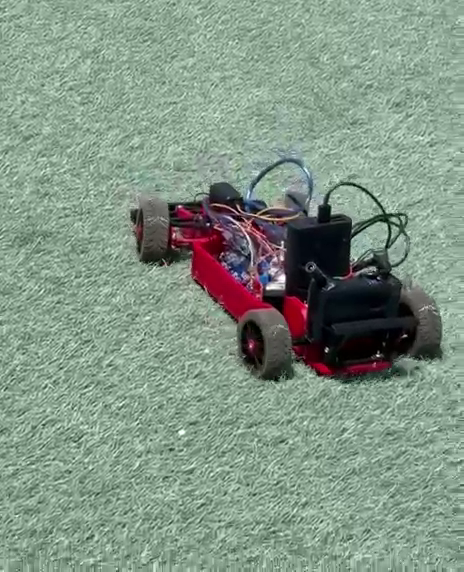
\includegraphics[width=\linewidth]{figures/m2_hardware_actuator_test.png}
  \end{minipage}\hfill
  \begin{minipage}{0.34\columnwidth}
    \footnotesize
    \textbf{Pi 4 host}\\
    \textbf{Pico} RP2040\\
    \textbf{Drive} L298N + TT motor\\
    \textbf{Steering} MG995 servo\\
    \textbf{Sensing} encoder + MPU-6050\\
    \textbf{Loop} 50 Hz
  \end{minipage}
  \caption{Scaled vehicle platform used for the hardware demonstrations. The
  Pi hosts the ROS\,2 autonomy nodes, while the Pico closes the embedded
  actuation and sensing loop.}
  \label{fig:hardware_platform}
\end{figure}

\subsection{Validation Baseline}

Before autonomy behaviors were evaluated, the base software path was verified on
both the host-side Pi and the simulation workstation. The Pi-side
\texttt{ros2 doctor} run passed all five checks, and custom validation nodes
confirmed sustained ROS\,2 execution on both platforms. The Gazebo teleoperation
mode then confirmed that command publication, vehicle motion, and feedback
logging were all connected before the autonomy-specific nodes were introduced.
Figure~\ref{fig:validation_panel} condenses those bring-up artifacts into one
panel because their role in the final project is evidentiary, not narrative.

\begin{figure}[htbp]
  \centering
  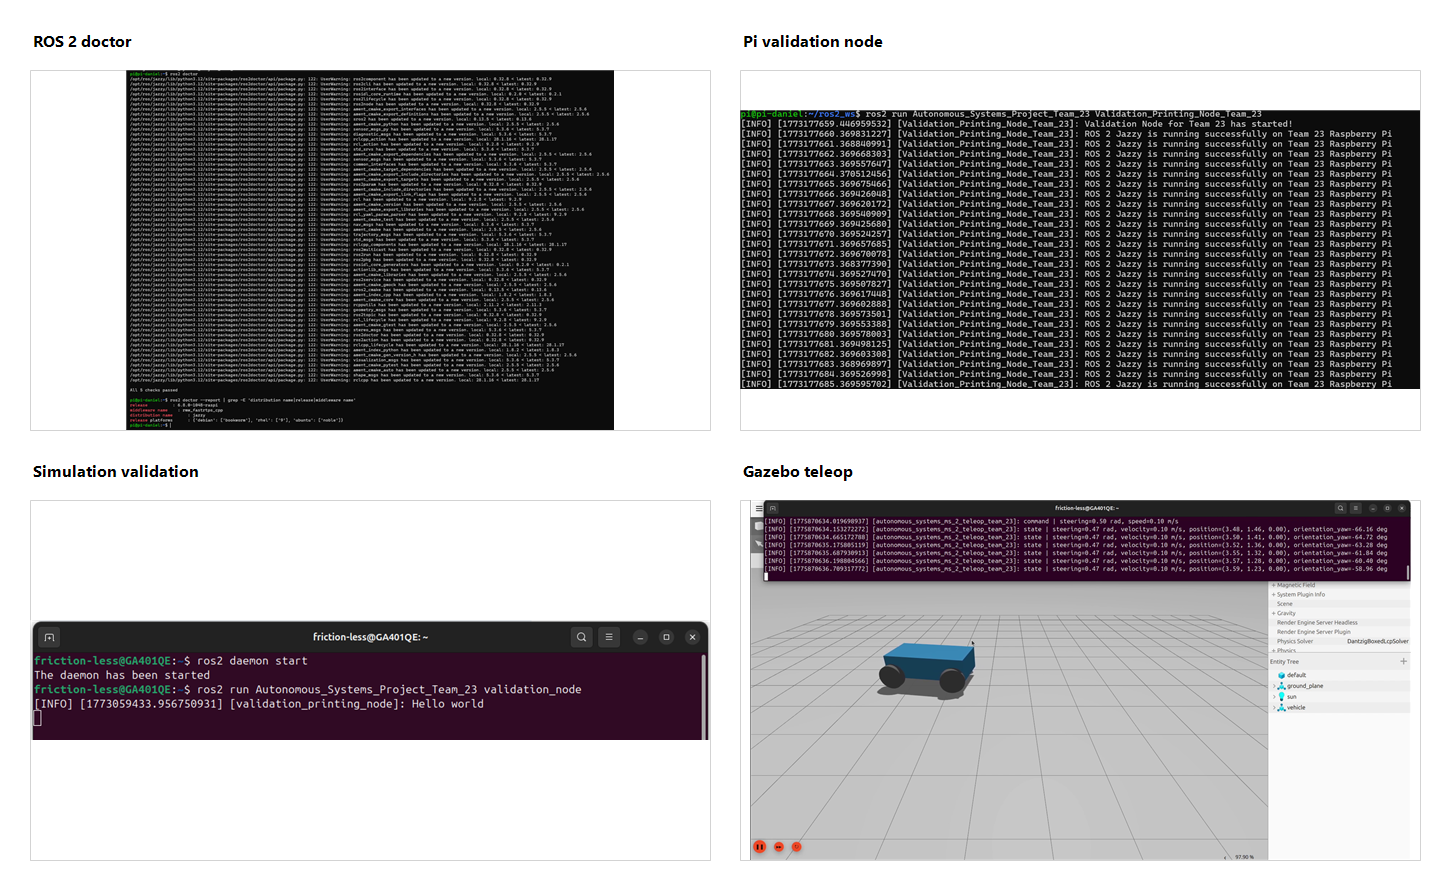
\includegraphics[width=\columnwidth]{figures/final_validation_panel.png}
  \caption{Condensed bring-up evidence: ROS\,2 diagnostics on the Raspberry
  Pi, hardware and simulation validation nodes, and Gazebo teleoperation for the
  initial motion and feedback path.}
  \label{fig:validation_panel}
\end{figure}

\subsection{Track Scenarios and Final Parameters}

The final autonomy stack was exercised on three predefined scenarios: a straight
track, a two-lane racing track with fixed obstacles, and a city-style track with
repeated turns. Table~\ref{tab:runtime_parameters} lists the runtime parameters
that matter most for interpreting the results.

\begin{table}[htbp]
  \caption{Key Runtime Parameters in the Final Integrated Stack}
  \label{tab:runtime_parameters}
  \centering
  \scriptsize
  \resizebox{\columnwidth}{!}{%
  \begin{tabular}{lll}
    \toprule
    Group & Item & Value \\
    \midrule
    Vehicle & Wheelbase & 0.255 m \\
    Vehicle & Pico control loop & 50 Hz \\
    Planner & Straight-track speed & 0.50 m/s \\
    Planner & Racing straight / lane-change speed & 0.26 / 0.14 m/s \\
    Planner & City straight / turn speed & 0.35 / 0.18 m/s \\
    Control & Speed PID & 0.85, 0.10, 0.03 \\
    Control & Stanley / heading & 0.30; 0.50 / 0.15 \\
    Loc. & Meas. std $(x,y,\theta,v,\omega)$ & 0.03, 0.03, 0.04, 0.05, 0.08 \\
    Loc. & Proc. std $(v,\omega)$ & 0.025, 0.05 \\
    \bottomrule
  \end{tabular}
  }
\end{table}

\section{Planning, Control, and Localization}
\label{sec:methods}

\subsection{Longitudinal and Lateral Control}

The longitudinal controller is a standard discrete PID loop that tracks the
planner's desired speed:

\begin{equation}
  u(t) = K_p e(t) + K_i \int_0^t e(\tau)\,d\tau + K_d \frac{de(t)}{dt},
  \label{eq:pid_speed}
\end{equation}

where $e(t)$ is the speed error. The lateral controller is best described as a
Stanley-style controller rather than a textbook Stanley implementation because
the shipped node combines heading error, a Stanley cross-track term, integral
bias correction, and yaw-rate damping:

\begin{equation}
  \delta = K_{\psi} e_{\psi} + \arctan\!\left(\frac{k_y e_y}{\max(|v|, v_0)}\right)
  + K_I \int e_y\,dt - K_d \dot{\psi},
  \label{eq:stanley_style}
\end{equation}

where $e_{\psi}$ is heading error, $e_y$ is cross-track error, and $v_0$
softens the low-speed response. This form matches the node that was ultimately
launched in the final stack and is more precise than calling the implementation
a pure Stanley controller.

\subsection{Track Planner}

The planner publishes desired speed, desired lane, and desired heading targets.
On the straight track, it mainly acts as a centerline and stop-state generator.
On the racing track, it applies a geometry-aware lane profile that starts in the
left lane, transitions right early enough to clear a fixed obstacle, and then
returns left for the second obstacle. The exported racing-track evaluation uses a
scheduled speed reduction from 0.26~m/s on straights to 0.14~m/s during lane
changes. On the city track, the planner similarly reduces the target speed from
0.35~m/s on straights to 0.18~m/s in the repeated-turn segments.

\subsection{Kalman-Filter Localization}

The final localization node operates on the state
$\mathbf{x} = [x, y, \theta, v, \omega]^\top$. During simulation-side
evaluation, it subscribes to Gazebo's ideal odometry, injects white Gaussian
noise using the standard deviations listed in
Table~\ref{tab:runtime_parameters}, and then applies a linearized discrete
Kalman filter. The motion model retains the Ackermann-inspired kinematic
structure through the yaw-rate relationship

\begin{equation}
  \dot{\psi} = \frac{v \tan\delta}{L},
  \label{eq:yaw_rate}
\end{equation}

while the filter predicts and corrects the state with the standard linear
Kalman recursion. The value of this node in the final project is twofold: it
provides a filtered \texttt{/odom} topic that the planner and controllers can
share, and it also exports the CSV and PNG artifacts used for the quantitative
evaluation in Section~\ref{sec:results}.

\section{Results}
\label{sec:results}

\subsection{From Bring-Up to Integrated Execution}

The validation evidence in Fig.~\ref{fig:validation_panel} confirms that the
project foundation is real rather than implied: the Raspberry Pi installation
passes all five \texttt{ros2 doctor} checks, custom validation nodes run on both
platforms, and Gazebo teleoperation closes the early command-feedback loop. This
baseline matters because the later autonomy behaviors are only meaningful once
that communication path is stable.

\subsection{Straight-Track State Tracking Under Injected Noise}

Figure~\ref{fig:track1_overview} shows the exported straight-track MS5 artifact
over a 10.34~s run. In this scenario, the noisy state has a position RMSE of
4.17~cm relative to the ideal trajectory, while the filtered estimate reduces
that error to 0.71~cm. Heading RMSE drops from $2.19^{\circ}$ to
$0.42^{\circ}$, and speed RMSE drops from 0.0495~m/s to 0.0243~m/s. The key
point is not only that the filter smooths the curves, but that the straight
track keeps model mismatch low enough for the prediction step to meaningfully
regularize each noisy update.

The filtered lateral deviation on the straight track is 0.0034~m RMS, with a
0.0218~m peak absolute deviation relative to the ideal centerline. That small
lateral error is consistent with the simple geometry of the track and explains
why the stack is able to use the straight-track scenario as a sanity check for
the full pipeline before more aggressive maneuvering.

\begin{figure}[htbp]
  \centering
  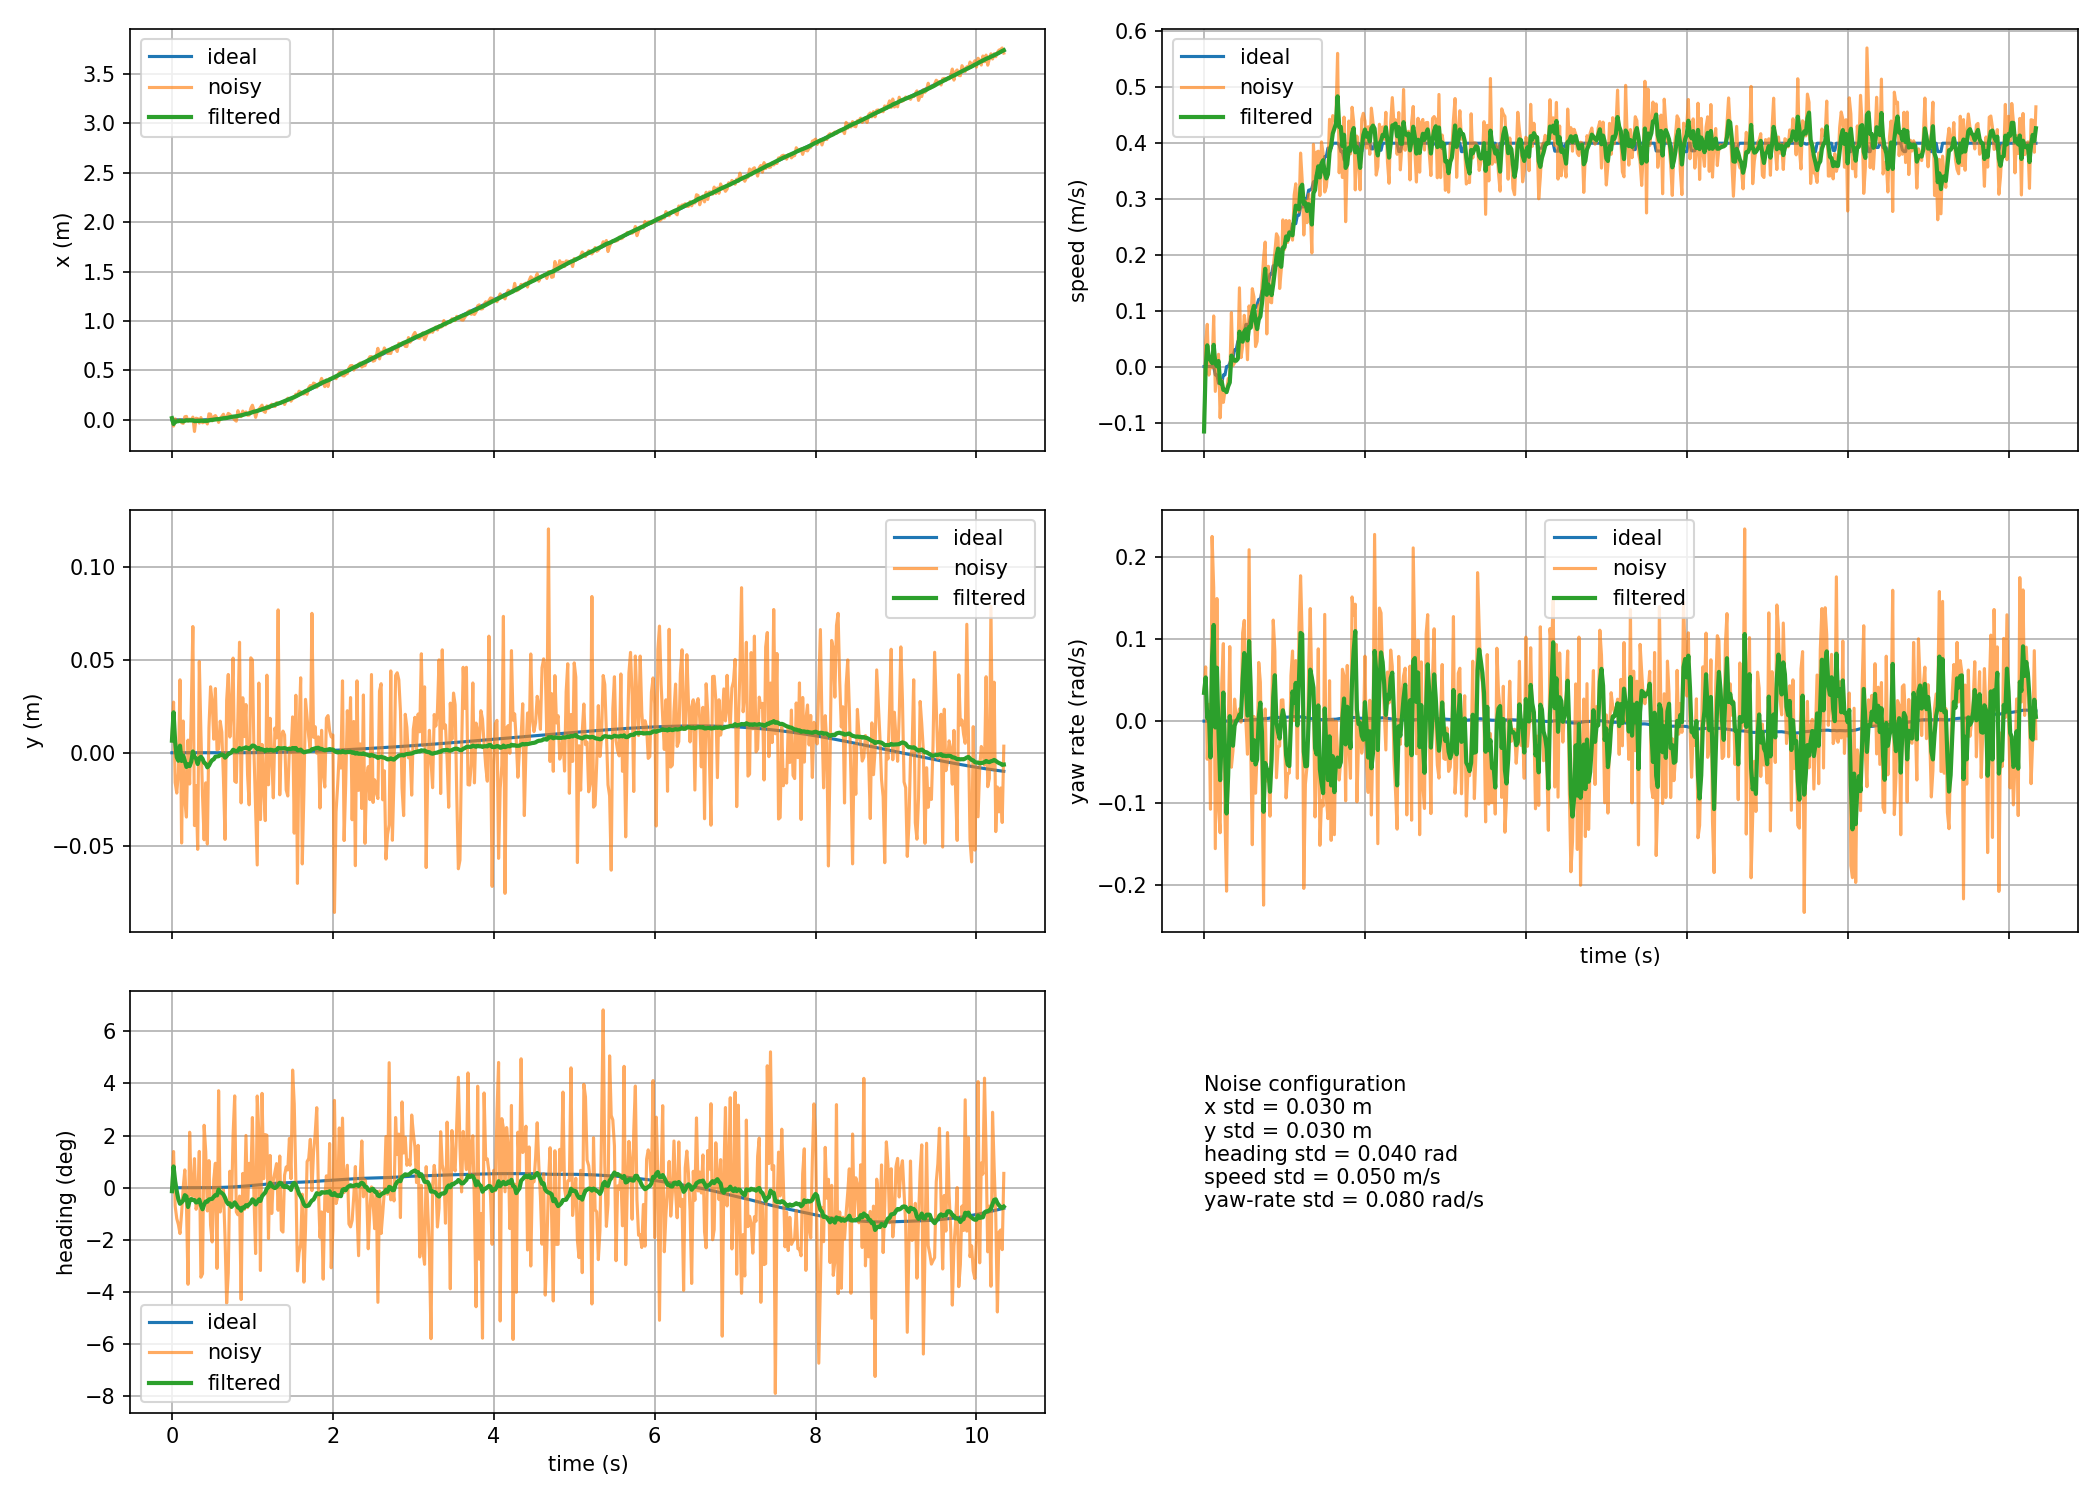
\includegraphics[width=\columnwidth]{figures/ms5_track1_overview.png}
  \caption{Exported MS5 straight-track artifact. The filtered states follow the
  ideal $x$, $y$, heading, speed, and yaw-rate histories much more closely than
  the noisy measurements over the 10.34~s run.}
  \label{fig:track1_overview}
\end{figure}

\subsection{Racing-Track Path Following and Localization}

The racing-track artifact is more revealing because it exercises both lane
changes and localization simultaneously. The planner lowers the target speed to
0.14~m/s during lane transitions and restores 0.26~m/s on straights. The result
should be interpreted as path-following performance under that scheduled
profile, not as an isolated ablation proving that the speed reduction alone
caused the improvement.

Figure~\ref{fig:racing_path} shows the corresponding XY path. The filtered path
remains close to the ideal lane-change corridor while the noisy path spreads
more widely around it. Quantitatively, the racing scenario improves from
4.17~cm to 0.69~cm position RMSE and from $2.19^{\circ}$ to $0.42^{\circ}$
heading RMSE. Filtered lateral error drops to 0.0026~m RMS. Because the same
noise configuration and filter structure are used on both the straight and
racing cases, the near-identical RMSE reduction indicates that the localization
benefit is robust across at least two distinct path geometries, not only one
special-case run.

\begin{figure}[htbp]
  \centering
  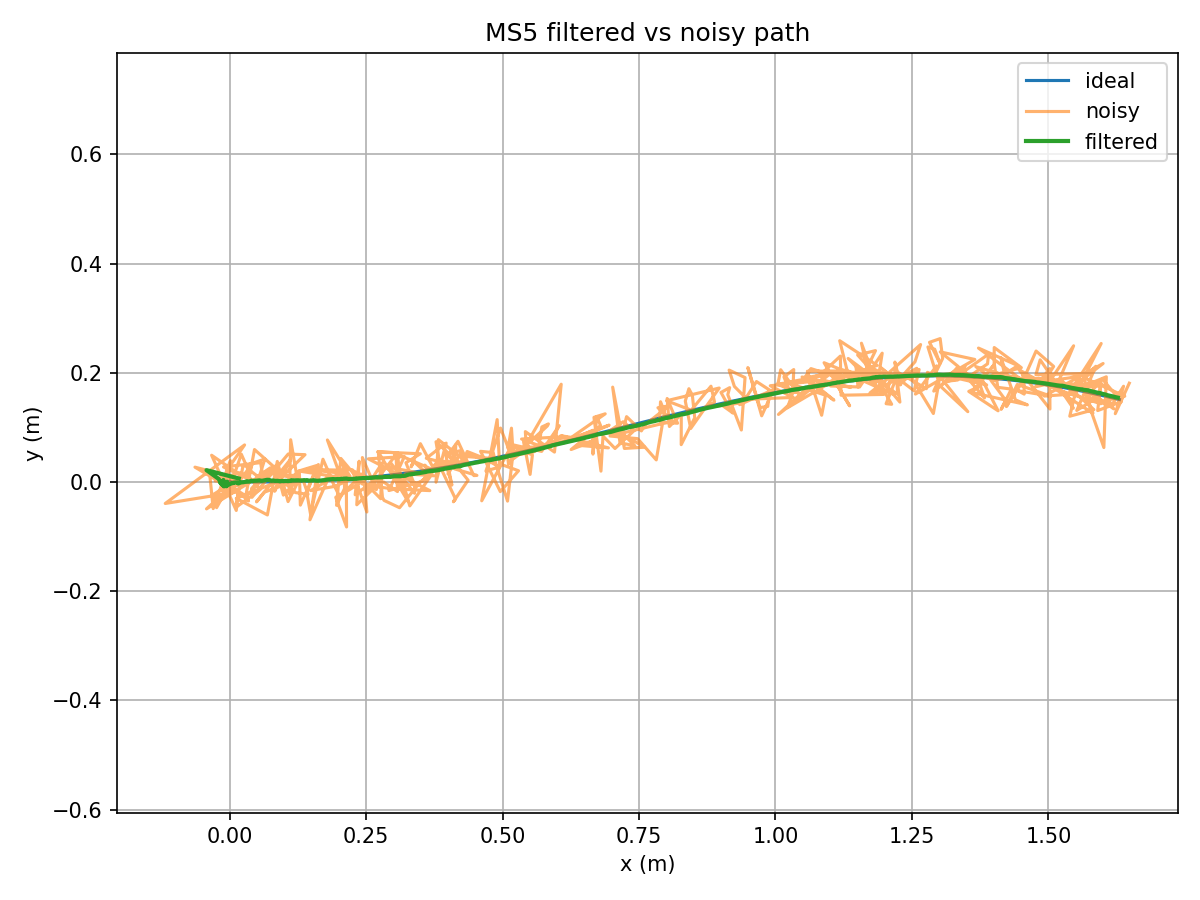
\includegraphics[width=\columnwidth]{figures/ms5_racing_xy_path.png}
  \caption{Exported MS5 racing-track XY path. The filtered trajectory stays
  near the ideal lane-change corridor through the obstacle-avoidance sequence,
  while the noisy path diverges more visibly.}
  \label{fig:racing_path}
\end{figure}

Table~\ref{tab:rmse_summary} and Fig.~\ref{fig:rmse_chart} summarize the
source-backed quantitative gains that can be claimed from the available course
artifacts.

\begin{table}[htbp]
  \caption{MS5 Localization Improvements from Exported CSV Artifacts}
  \label{tab:rmse_summary}
  \centering
  \footnotesize
  \begin{tabular}{@{}lccc@{}}
    \toprule
    Scenario & Pos. gain & Heading gain & Speed gain \\
    \midrule
    Straight track & 82.9\% & 81.0\% & 51.0\% \\
    Racing track & 83.5\% & 80.7\% & 47.2\% \\
    \bottomrule
  \end{tabular}
\end{table}

\begin{figure}[htbp]
  \centering
  \begin{tikzpicture}
    \begin{groupplot}[
      group style={group size=2 by 1, horizontal sep=1.1cm},
      width=0.22\textwidth,
      height=0.16\textheight,
      ybar,
      ymin=0,
      symbolic x coords={Straight,Racing},
      xtick=data,
      xticklabel style={font=\scriptsize},
      ylabel style={font=\scriptsize},
      title style={font=\footnotesize},
      legend style={font=\scriptsize, draw=none, at={(0.5,1.18)}, anchor=south, legend columns=2},
      nodes near coords,
      every node near coord/.append style={font=\scriptsize},
      enlarge x limits=0.28
    ]
      \nextgroupplot[
        title={Position RMSE},
        ylabel={m}
      ]
      \addplot[fill=gray!45] coordinates {(Straight,0.0417) (Racing,0.0417)};
      \addplot[fill=blue!55] coordinates {(Straight,0.0071) (Racing,0.0069)};
      \legend{Noisy, Filtered}

      \nextgroupplot[
        title={Heading RMSE},
        ylabel={deg}
      ]
      \addplot[fill=gray!45] coordinates {(Straight,2.19) (Racing,2.19)};
      \addplot[fill=blue!55] coordinates {(Straight,0.42) (Racing,0.42)};
    \end{groupplot}
  \end{tikzpicture}
  \caption{Absolute RMSE values from the exported MS5 artifacts. The Kalman
  filter consistently reduces both position and heading error across the two
  evaluated scenarios.}
  \label{fig:rmse_chart}
\end{figure}

\subsection{Final Integrated Autonomy Demonstrations}

The available hardware evidence is qualitative rather than numeric, but it still
matters because it validates the final system boundary claimed in this work. The
hardware run in Fig.~\ref{fig:autonomy_panel} shows that the onboard Pi and Pico
stack can execute a representative predefined autonomy demonstration without a
GUI-driven operator. The paired MS5 node graph confirms that localization,
planning, and control were composed as one ROS\,2 pipeline rather than as
disconnected milestone scripts.

What cannot be claimed from the available hardware artifacts is scenario-by-
scenario hardware benchmarking or real-world RMSE, because the course folder
contains images and videos for the demonstrations but not synchronized hardware
log files with ground truth. The final report therefore treats hardware autonomy
as demonstrated qualitatively, while the quantitative comparisons in this paper
remain tied to the exported MS5 simulation artifacts.

\begin{figure}[htbp]
  \centering
  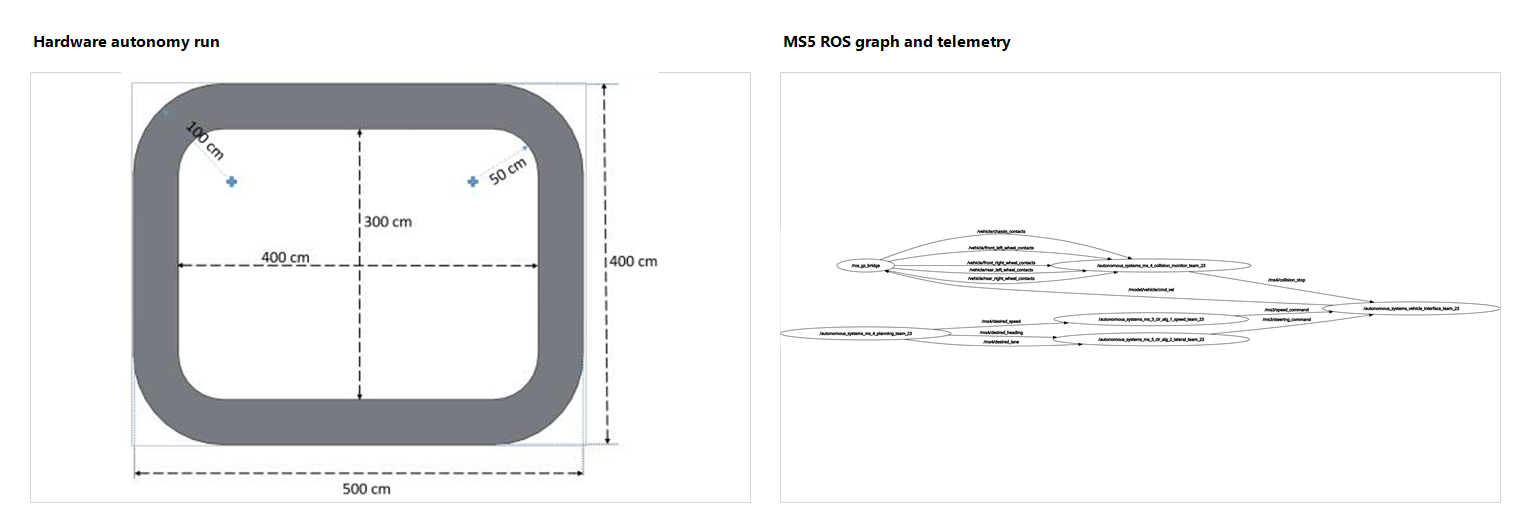
\includegraphics[width=\columnwidth]{figures/final_autonomy_panel.png}
  \caption{Final integrated autonomy evidence assembled from course artifacts:
  a physical headless autonomy run and the MS5 ROS\,2 node graph / telemetry
  environment used to validate the full pipeline.}
  \label{fig:autonomy_panel}
\end{figure}

\section{Discussion and Limitations}
\label{sec:discussion}

\textbf{The main contribution is integration, not any single node.}
The strongest result of the project is that the same ROS\,2 command-state
interfaces survive the full trip from Gazebo validation to embedded actuation and
back to filtered odometry. This is why the project is more valuable than a ROS
installation checklist: the planner, controllers, and localization node are all
exercised as one autonomy stack.

\textbf{The racing-track result should be read as performance under a scheduled
planner profile, not as a speed-scheduling ablation.}
The lane-change speed reduction from 0.26~m/s to 0.14~m/s is part of the
documented planner configuration. On a 0.255~m wheelbase vehicle, that slower
profile is a plausible design choice, and it is consistent with the clean path
shown in Fig.~\ref{fig:racing_path}. What the available artifacts do not prove
in isolation is how much of the improvement is attributable to speed scheduling
alone versus the rest of the controller-and-estimator stack.

\textbf{The localization gains are real but bounded by the evaluation setup.}
The reported RMSE improvements come from the exported MS5 simulation runs where
noise is injected into Gazebo odometry and then filtered. That setup is still
useful because it reveals the effect of the estimator under known conditions, but
it should not be confused with a hardware-ground-truth benchmark.

\textbf{The central limitation is track-bounded autonomy with limited sensing.}
The planner assumes known tracks and fixed obstacle geometry. The hardware stack
uses proprioceptive sensing only: encoder and IMU data. As a result, the system
does not perceive unexpected obstacles, does not replan around dynamic agents,
and does not perform SLAM in unknown environments. A second limitation is that
the course artifacts do not include synchronized hardware logs against an
external reference, so real-world localization error cannot be quantified
honestly from the available material.

\section{Conclusion}
\label{sec:conclusion}

This paper reframed Team~23's autonomous systems project as a final integrated
Ackermann autonomy stack instead of a milestone chronology. The resulting system
links ROS\,2 Jazzy, Gazebo Harmonic, shared planning and control nodes,
Pico-based embedded actuation, and Kalman-filtered localization across straight,
racing, and city-style demonstrations. The strongest quantitative evidence comes
from the exported MS5 artifacts, where the localization node reduces position
RMSE by about 83\% and heading RMSE by about 81\% under the documented noise
conditions. The strongest practical evidence is that the same stack runs through
to a representative headless hardware demonstration. The remaining gap is equally clear: the
current project is a known-track autonomy pipeline with limited sensing, not a
generalized perception-rich autonomous vehicle.

\section*{Acknowledgment}

The authors thank Dr. Omar M. Shehata and Eng. Dalia M. Mahfouz for their
guidance and support throughout the MCTR~1002 Autonomous Systems course project.

\bibliographystyle{IEEEtran}
\bibliography{references}

\end{document}
